\section{Evaluation}

This section evaluates the performance of our approach to mine cultural differences of named entities from large text.
First of all, we introduce the details in building the English and
Chinese corpus.
Then, we present how we construct the ground truth from human annotation.
Finally, we report the evaluation metrics we use to evaluate our approach
as well as the experiment results.

\subsection{Data Preparation}
\label{sec:dataeval}
To build English corpus, we  crawled news articles from Daily Mail and New York Times
published between Jan 1st, 2012 to Aug 5th, 2016, for these two sources
are among the most representative news media of western cultures.
Similarly, we crawled China News
and iFeng News in the same time period to build our Chinese corpus.
In total, there are 1,857,581 English news and 673,655 Chinese news.
An average English news has 558.2 words while the average length of a
Chinese news is 507.3 words.\footnote{Our vocabulary contains 45,740 English terms and
	47,854 Chinese terms,  including 4,212 terms representing the
	named entities common to two term sets.
	For the purpose of implementing the Translation Space algorithm,
	we build 122,284 translation pairs between the two term sets.}

\subsection{Ground Truth}

As shown in \secref{sec:intro}, cultural differences of a given entity
is visible from the most popular images in the image search results.
It is because that people from different cultures have different views
on the same entity so the kind of images that they search or create
on the Internet are very different, too.
With the help of the online image search engine such as Bing,
we can get the most interesting images of a given named entity
in western culture with Bing's global
site and in Chinese culture
with its Chinese site.
%\BL{Put the global url and cn url later}.

%Due to this fact, we consider using the

%
%To determine the ground truth determining whether
%the given entity has cultural difference,
%%that a pair of terms is culturally different or not,
%%we get help from Bing image search.
%we adopt Bing image search results.
%We believe that if an entity has cultural differences,
%such differences should be reflected in the choice of using images in the documents on such entity.
%As a result, highly ranked images from commercial search engines reflect dominant perception
%of the given entity in the culture.
%such that representative perception in the given culture is reflected in the highly ranked pictures in commercial
%search engines.
%This argument is evident in examples shown in Section 1: Kashmir is more frequently described with scenic photos
%in English documents, and with military pictures in Chinese documents.


Thus, we obtain manual labels of 885 named
entities by
%intervention to annotate such difference:
%We build
showing human annotators the top 20 pictures of a certain
named entity from global Bing image search and the Chinese Bing image
search respectively.
This set of 885 entities is the intersection of the 2000 most frequent
entities in the English corpus and Chinese corpus respectively.
We invited 14 annotators from different cultures (both Chinese and
international students) to judge whether the two sets of image search results
of a given entity are visually different, without considering the actual
meaning of the entity.

%\HY{give an example to show different and same respectively}
%Finally, we treat a named entity as culturally different, only if at least 60\% of the annotators think so ,
%and consider a named entity as culturally similar only if at least 80\% of human annotators agrees it.
%Then we filter out other entities out of this boundary.
%\SH{XX\% of entities satisfy such condition and thus ensure kappa agreement score above YY}.
%Those not satisfying such condition are considered controversial and pruned out.

We choose 497 entities that most annotator agree on as
our evaluation ground truth. The inter-annotator  agreement by
Cohen's kappa coefficient among these annotator is 0.6.
Among these annotated pairs,
we set aside 100 entities for which all annotators consider culturally similar.
These are used as the training set for the linear transformation model.
Consequently, our final test dataset consists of 397 entities,
out of which 173 are labeled as culturally different and 224 labeled
as culturally similar. Considering the percentage of annotators who label each pair as similar, we obtain the scores of each entity. 
Thus, we propose a ranking-based evaluation to investigate the performance of our method.

\subsection{Baselines}
We compare our approach with two baseline methods:

\subsubsection{Biased Random Classifier}
To judge whether a named entity is culturally different or not is
actually a classification problem.
Thus, a biased random classifier with a prior probability computed by
the ratio of the number of culturally different entities to
the total number of entities in the training data can be
a simple baseline.

\subsubsection{Ranking by Popularity}
A stronger baseline is to rank the entities in test dataset by the sum of the relative frequency of
this entity in the English corpus and Chinese corpus.
\footnote{The reason why it is stronger than the former one is that when a named entity is more likely to occur in different cultures, it has more chance to be viewed in different ways.
If an object is not very common in different cultures, it has almost no opportunity to be
exposed to multiple cultural views.
%known in multiple ways. Thus,
Based on this assumption, we consider this baseline is a stronger competitor to our two algorithms.}  

\begin{figure*}[th!]
	\label{fig:atk}
	\begin{subfigure}{0.67\columnwidth}
		\resizebox{\columnwidth}{!}{% GNUPLOT: LaTeX picture with Postscript
\begingroup
  \makeatletter
  \providecommand\color[2][]{%
    \GenericError{(gnuplot) \space\space\space\@spaces}{%
      Package color not loaded in conjunction with
      terminal option `colourtext'%
    }{See the gnuplot documentation for explanation.%
    }{Either use 'blacktext' in gnuplot or load the package
      color.sty in LaTeX.}%
    \renewcommand\color[2][]{}%
  }%
  \providecommand\includegraphics[2][]{%
    \GenericError{(gnuplot) \space\space\space\@spaces}{%
      Package graphicx or graphics not loaded%
    }{See the gnuplot documentation for explanation.%
    }{The gnuplot epslatex terminal needs graphicx.sty or graphics.sty.}%
    \renewcommand\includegraphics[2][]{}%
  }%
  \providecommand\rotatebox[2]{#2}%
  \@ifundefined{ifGPcolor}{%
    \newif\ifGPcolor
    \GPcolortrue
  }{}%
  \@ifundefined{ifGPblacktext}{%
    \newif\ifGPblacktext
    \GPblacktextfalse
  }{}%
  % define a \g@addto@macro without @ in the name:
  \let\gplgaddtomacro\g@addto@macro
  % define empty templates for all commands taking text:
  \gdef\gplbacktext{}%
  \gdef\gplfronttext{}%
  \makeatother
  \ifGPblacktext
    % no textcolor at all
    \def\colorrgb#1{}%
    \def\colorgray#1{}%
  \else
    % gray or color?
    \ifGPcolor
      \def\colorrgb#1{\color[rgb]{#1}}%
      \def\colorgray#1{\color[gray]{#1}}%
      \expandafter\def\csname LTw\endcsname{\color{white}}%
      \expandafter\def\csname LTb\endcsname{\color{black}}%
      \expandafter\def\csname LTa\endcsname{\color{black}}%
      \expandafter\def\csname LT0\endcsname{\color[rgb]{1,0,0}}%
      \expandafter\def\csname LT1\endcsname{\color[rgb]{0,1,0}}%
      \expandafter\def\csname LT2\endcsname{\color[rgb]{0,0,1}}%
      \expandafter\def\csname LT3\endcsname{\color[rgb]{1,0,1}}%
      \expandafter\def\csname LT4\endcsname{\color[rgb]{0,1,1}}%
      \expandafter\def\csname LT5\endcsname{\color[rgb]{1,1,0}}%
      \expandafter\def\csname LT6\endcsname{\color[rgb]{0,0,0}}%
      \expandafter\def\csname LT7\endcsname{\color[rgb]{1,0.3,0}}%
      \expandafter\def\csname LT8\endcsname{\color[rgb]{0.5,0.5,0.5}}%
    \else
      % gray
      \def\colorrgb#1{\color{black}}%
      \def\colorgray#1{\color[gray]{#1}}%
      \expandafter\def\csname LTw\endcsname{\color{white}}%
      \expandafter\def\csname LTb\endcsname{\color{black}}%
      \expandafter\def\csname LTa\endcsname{\color{black}}%
      \expandafter\def\csname LT0\endcsname{\color{black}}%
      \expandafter\def\csname LT1\endcsname{\color{black}}%
      \expandafter\def\csname LT2\endcsname{\color{black}}%
      \expandafter\def\csname LT3\endcsname{\color{black}}%
      \expandafter\def\csname LT4\endcsname{\color{black}}%
      \expandafter\def\csname LT5\endcsname{\color{black}}%
      \expandafter\def\csname LT6\endcsname{\color{black}}%
      \expandafter\def\csname LT7\endcsname{\color{black}}%
      \expandafter\def\csname LT8\endcsname{\color{black}}%
    \fi
  \fi
    \setlength{\unitlength}{0.0500bp}%
    \ifx\gptboxheight\undefined%
      \newlength{\gptboxheight}%
      \newlength{\gptboxwidth}%
      \newsavebox{\gptboxtext}%
    \fi%
    \setlength{\fboxrule}{0.5pt}%
    \setlength{\fboxsep}{1pt}%
\begin{picture}(5040.00,3772.00)%
    \gplgaddtomacro\gplbacktext{%
      \csname LTb\endcsname%
      \put(666,576){\makebox(0,0)[r]{\strut{}$0$}}%
      \put(666,1172){\makebox(0,0)[r]{\strut{}$0.2$}}%
      \put(666,1768){\makebox(0,0)[r]{\strut{}$0.4$}}%
      \put(666,2363){\makebox(0,0)[r]{\strut{}$0.6$}}%
      \put(666,2959){\makebox(0,0)[r]{\strut{}$0.8$}}%
      \put(666,3555){\makebox(0,0)[r]{\strut{}$1$}}%
      \put(774,396){\makebox(0,0){\strut{}$0$}}%
      \put(1329,396){\makebox(0,0){\strut{}$100$}}%
      \put(1884,396){\makebox(0,0){\strut{}$200$}}%
      \put(2439,396){\makebox(0,0){\strut{}$300$}}%
      \put(2994,396){\makebox(0,0){\strut{}$400$}}%
      \put(3549,396){\makebox(0,0){\strut{}$500$}}%
      \put(4104,396){\makebox(0,0){\strut{}$600$}}%
      \put(4659,396){\makebox(0,0){\strut{}$700$}}%
    }%
    \gplgaddtomacro\gplfronttext{%
      \csname LTb\endcsname%
      \put(144,2065){\rotatebox{-270}{\makebox(0,0){\strut{}precision at $k$}}}%
      \put(2744,126){\makebox(0,0){\strut{}top $k$}}%
      \csname LTb\endcsname%
      \put(3896,3402){\makebox(0,0)[r]{\strut{}BL-JS}}%
      \csname LTb\endcsname%
      \put(3896,3222){\makebox(0,0)[r]{\strut{}WN-JS}}%
      \csname LTb\endcsname%
      \put(3896,3042){\makebox(0,0)[r]{\strut{}EM-JS}}%
      \csname LTb\endcsname%
      \put(3896,2862){\makebox(0,0)[r]{\strut{}LinearTrans}}%
      \csname LTb\endcsname%
      \put(3896,2682){\makebox(0,0)[r]{\strut{}BiLexTrans}}%
      \csname LTb\endcsname%
      \put(3896,2502){\makebox(0,0)[r]{\strut{}SocVec:opn}}%
      \csname LTb\endcsname%
      \put(3896,2322){\makebox(0,0)[r]{\strut{}SocVec:all}}%
    }%
    \gplbacktext
    \put(0,0){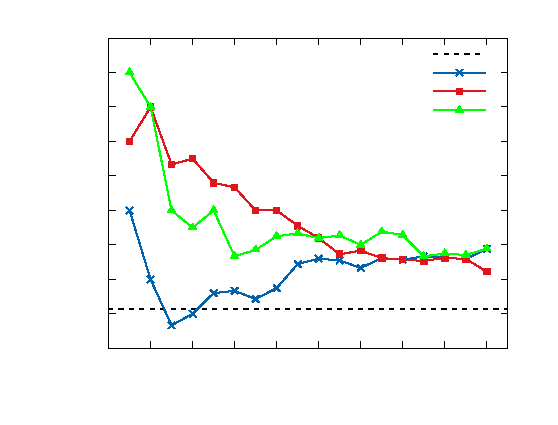
\includegraphics{precisionatk}}%
    \gplfronttext
  \end{picture}%
\endgroup
}
		\caption{Precision at top $k$}
		\label{fig:precisionatk}
	\end{subfigure}
	\hfill
	\begin{subfigure}{0.67\columnwidth}
		\resizebox{\columnwidth}{!}{% GNUPLOT: LaTeX picture with Postscript
\begingroup
  \makeatletter
  \providecommand\color[2][]{%
    \GenericError{(gnuplot) \space\space\space\@spaces}{%
      Package color not loaded in conjunction with
      terminal option `colourtext'%
    }{See the gnuplot documentation for explanation.%
    }{Either use 'blacktext' in gnuplot or load the package
      color.sty in LaTeX.}%
    \renewcommand\color[2][]{}%
  }%
  \providecommand\includegraphics[2][]{%
    \GenericError{(gnuplot) \space\space\space\@spaces}{%
      Package graphicx or graphics not loaded%
    }{See the gnuplot documentation for explanation.%
    }{The gnuplot epslatex terminal needs graphicx.sty or graphics.sty.}%
    \renewcommand\includegraphics[2][]{}%
  }%
  \providecommand\rotatebox[2]{#2}%
  \@ifundefined{ifGPcolor}{%
    \newif\ifGPcolor
    \GPcolortrue
  }{}%
  \@ifundefined{ifGPblacktext}{%
    \newif\ifGPblacktext
    \GPblacktextfalse
  }{}%
  % define a \g@addto@macro without @ in the name:
  \let\gplgaddtomacro\g@addto@macro
  % define empty templates for all commands taking text:
  \gdef\gplbacktext{}%
  \gdef\gplfronttext{}%
  \makeatother
  \ifGPblacktext
    % no textcolor at all
    \def\colorrgb#1{}%
    \def\colorgray#1{}%
  \else
    % gray or color?
    \ifGPcolor
      \def\colorrgb#1{\color[rgb]{#1}}%
      \def\colorgray#1{\color[gray]{#1}}%
      \expandafter\def\csname LTw\endcsname{\color{white}}%
      \expandafter\def\csname LTb\endcsname{\color{black}}%
      \expandafter\def\csname LTa\endcsname{\color{black}}%
      \expandafter\def\csname LT0\endcsname{\color[rgb]{1,0,0}}%
      \expandafter\def\csname LT1\endcsname{\color[rgb]{0,1,0}}%
      \expandafter\def\csname LT2\endcsname{\color[rgb]{0,0,1}}%
      \expandafter\def\csname LT3\endcsname{\color[rgb]{1,0,1}}%
      \expandafter\def\csname LT4\endcsname{\color[rgb]{0,1,1}}%
      \expandafter\def\csname LT5\endcsname{\color[rgb]{1,1,0}}%
      \expandafter\def\csname LT6\endcsname{\color[rgb]{0,0,0}}%
      \expandafter\def\csname LT7\endcsname{\color[rgb]{1,0.3,0}}%
      \expandafter\def\csname LT8\endcsname{\color[rgb]{0.5,0.5,0.5}}%
    \else
      % gray
      \def\colorrgb#1{\color{black}}%
      \def\colorgray#1{\color[gray]{#1}}%
      \expandafter\def\csname LTw\endcsname{\color{white}}%
      \expandafter\def\csname LTb\endcsname{\color{black}}%
      \expandafter\def\csname LTa\endcsname{\color{black}}%
      \expandafter\def\csname LT0\endcsname{\color{black}}%
      \expandafter\def\csname LT1\endcsname{\color{black}}%
      \expandafter\def\csname LT2\endcsname{\color{black}}%
      \expandafter\def\csname LT3\endcsname{\color{black}}%
      \expandafter\def\csname LT4\endcsname{\color{black}}%
      \expandafter\def\csname LT5\endcsname{\color{black}}%
      \expandafter\def\csname LT6\endcsname{\color{black}}%
      \expandafter\def\csname LT7\endcsname{\color{black}}%
      \expandafter\def\csname LT8\endcsname{\color{black}}%
    \fi
  \fi
    \setlength{\unitlength}{0.0500bp}%
    \ifx\gptboxheight\undefined%
      \newlength{\gptboxheight}%
      \newlength{\gptboxwidth}%
      \newsavebox{\gptboxtext}%
    \fi%
    \setlength{\fboxrule}{0.5pt}%
    \setlength{\fboxsep}{1pt}%
\begin{picture}(5040.00,3772.00)%
    \gplgaddtomacro\gplbacktext{%
      \csname LTb\endcsname%
      \put(666,576){\makebox(0,0)[r]{\strut{}$0$}}%
      \put(666,1073){\makebox(0,0)[r]{\strut{}$0.1$}}%
      \put(666,1569){\makebox(0,0)[r]{\strut{}$0.2$}}%
      \put(666,2066){\makebox(0,0)[r]{\strut{}$0.3$}}%
      \put(666,2562){\makebox(0,0)[r]{\strut{}$0.4$}}%
      \put(666,3059){\makebox(0,0)[r]{\strut{}$0.5$}}%
      \put(666,3555){\makebox(0,0)[r]{\strut{}$0.6$}}%
      \put(774,396){\makebox(0,0){\strut{}$0$}}%
      \put(1189,396){\makebox(0,0){\strut{}$20$}}%
      \put(1604,396){\makebox(0,0){\strut{}$40$}}%
      \put(2019,396){\makebox(0,0){\strut{}$60$}}%
      \put(2433,396){\makebox(0,0){\strut{}$80$}}%
      \put(2848,396){\makebox(0,0){\strut{}$100$}}%
      \put(3263,396){\makebox(0,0){\strut{}$120$}}%
      \put(3678,396){\makebox(0,0){\strut{}$140$}}%
      \put(4093,396){\makebox(0,0){\strut{}$160$}}%
      \put(4508,396){\makebox(0,0){\strut{}$180$}}%
    }%
    \gplgaddtomacro\gplfronttext{%
      \csname LTb\endcsname%
      \put(144,2065){\rotatebox{-270}{\makebox(0,0){\strut{}recall at $k$}}}%
      \put(2744,126){\makebox(0,0){\strut{}top $k$}}%
      \csname LTb\endcsname%
      \put(1098,3402){\makebox(0,0)[r]{\strut{}ER}}%
      \csname LTb\endcsname%
      \put(1098,3222){\makebox(0,0)[r]{\strut{}PR}}%
      \csname LTb\endcsname%
      \put(1098,3042){\makebox(0,0)[r]{\strut{}LT}}%
      \csname LTb\endcsname%
      \put(1098,2862){\makebox(0,0)[r]{\strut{}TS}}%
    }%
    \gplbacktext
    \put(0,0){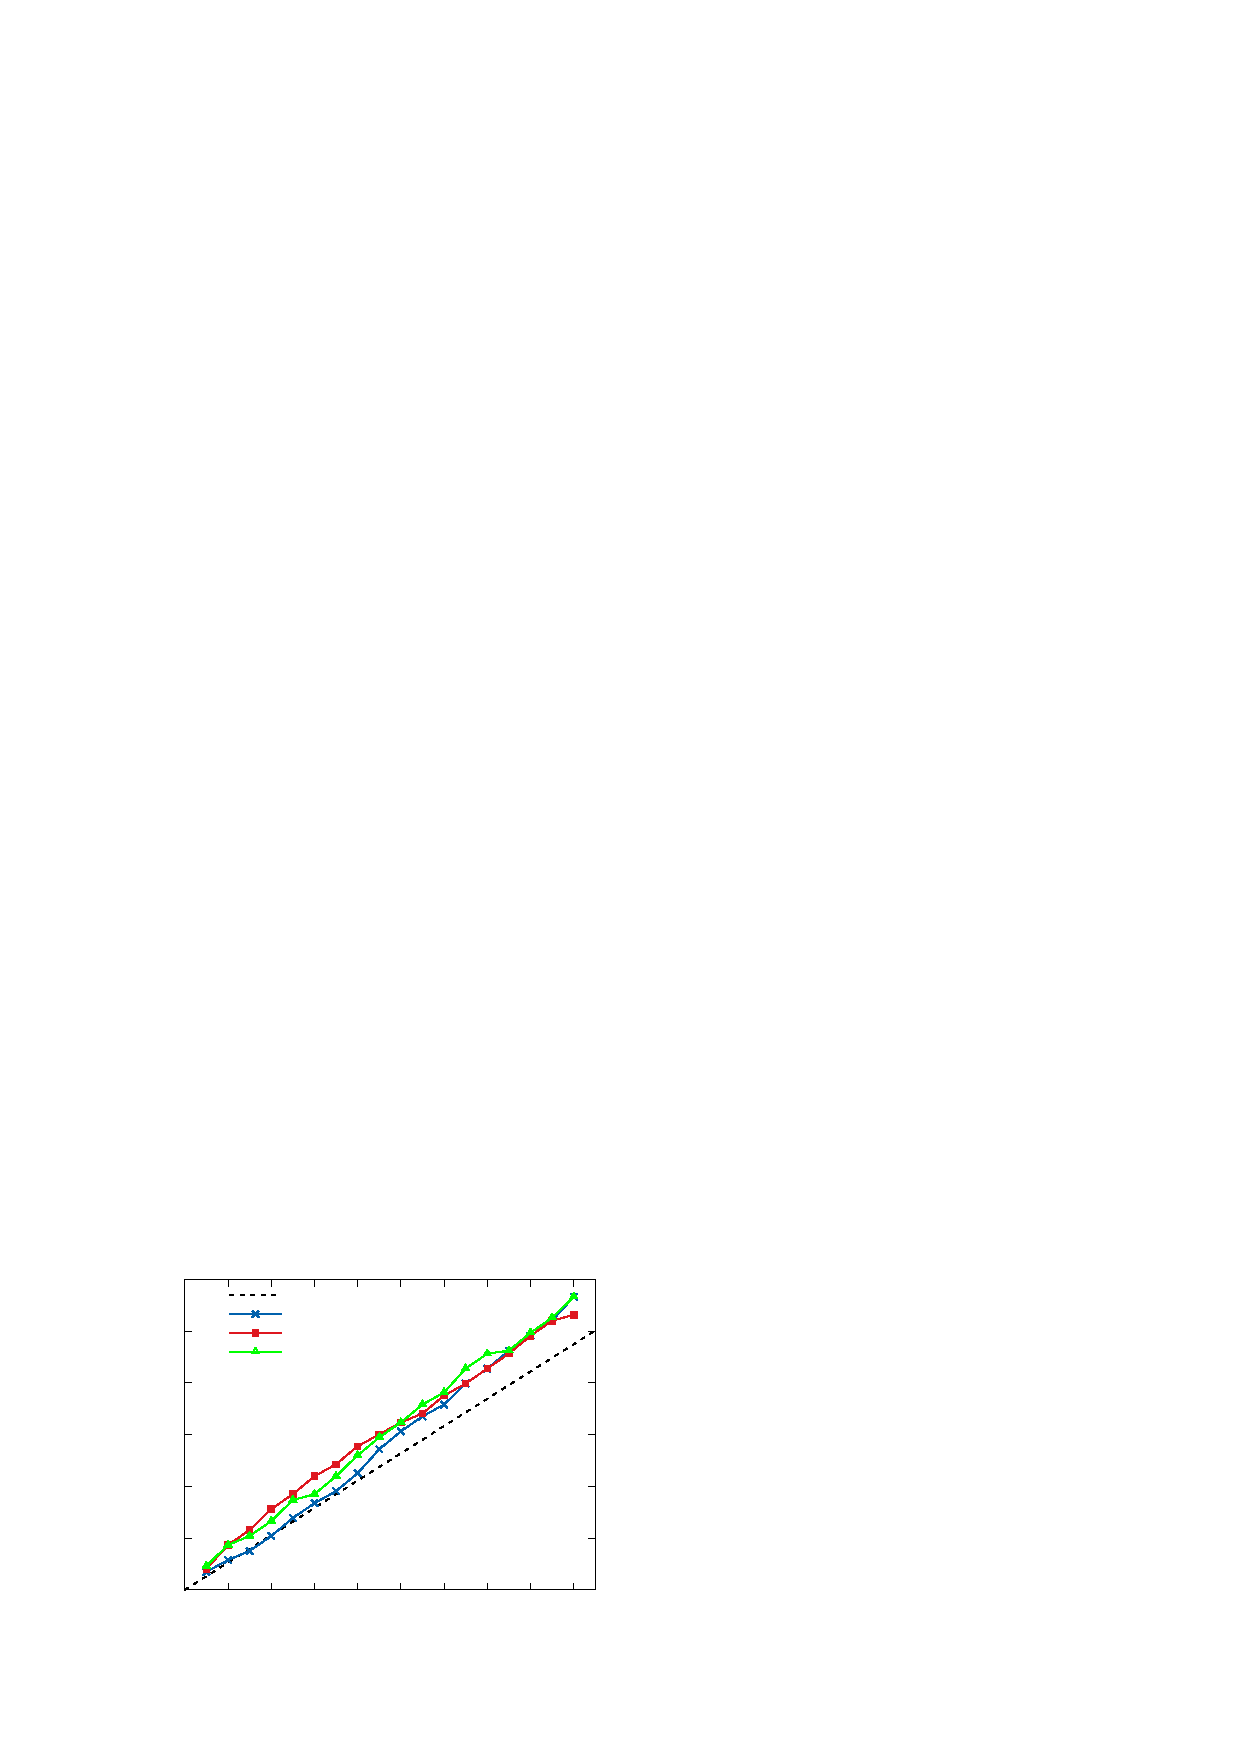
\includegraphics{recallatk}}%
    \gplfronttext
  \end{picture}%
\endgroup
}
		\caption{Recall at top $k$}
		\label{fig:recallatk}
	\end{subfigure}
	\hfill
	\begin{subfigure}{0.67\columnwidth}
		\resizebox{\columnwidth}{!}{% GNUPLOT: LaTeX picture with Postscript
\begingroup
  \makeatletter
  \providecommand\color[2][]{%
    \GenericError{(gnuplot) \space\space\space\@spaces}{%
      Package color not loaded in conjunction with
      terminal option `colourtext'%
    }{See the gnuplot documentation for explanation.%
    }{Either use 'blacktext' in gnuplot or load the package
      color.sty in LaTeX.}%
    \renewcommand\color[2][]{}%
  }%
  \providecommand\includegraphics[2][]{%
    \GenericError{(gnuplot) \space\space\space\@spaces}{%
      Package graphicx or graphics not loaded%
    }{See the gnuplot documentation for explanation.%
    }{The gnuplot epslatex terminal needs graphicx.sty or graphics.sty.}%
    \renewcommand\includegraphics[2][]{}%
  }%
  \providecommand\rotatebox[2]{#2}%
  \@ifundefined{ifGPcolor}{%
    \newif\ifGPcolor
    \GPcolortrue
  }{}%
  \@ifundefined{ifGPblacktext}{%
    \newif\ifGPblacktext
    \GPblacktextfalse
  }{}%
  % define a \g@addto@macro without @ in the name:
  \let\gplgaddtomacro\g@addto@macro
  % define empty templates for all commands taking text:
  \gdef\gplbacktext{}%
  \gdef\gplfronttext{}%
  \makeatother
  \ifGPblacktext
    % no textcolor at all
    \def\colorrgb#1{}%
    \def\colorgray#1{}%
  \else
    % gray or color?
    \ifGPcolor
      \def\colorrgb#1{\color[rgb]{#1}}%
      \def\colorgray#1{\color[gray]{#1}}%
      \expandafter\def\csname LTw\endcsname{\color{white}}%
      \expandafter\def\csname LTb\endcsname{\color{black}}%
      \expandafter\def\csname LTa\endcsname{\color{black}}%
      \expandafter\def\csname LT0\endcsname{\color[rgb]{1,0,0}}%
      \expandafter\def\csname LT1\endcsname{\color[rgb]{0,1,0}}%
      \expandafter\def\csname LT2\endcsname{\color[rgb]{0,0,1}}%
      \expandafter\def\csname LT3\endcsname{\color[rgb]{1,0,1}}%
      \expandafter\def\csname LT4\endcsname{\color[rgb]{0,1,1}}%
      \expandafter\def\csname LT5\endcsname{\color[rgb]{1,1,0}}%
      \expandafter\def\csname LT6\endcsname{\color[rgb]{0,0,0}}%
      \expandafter\def\csname LT7\endcsname{\color[rgb]{1,0.3,0}}%
      \expandafter\def\csname LT8\endcsname{\color[rgb]{0.5,0.5,0.5}}%
    \else
      % gray
      \def\colorrgb#1{\color{black}}%
      \def\colorgray#1{\color[gray]{#1}}%
      \expandafter\def\csname LTw\endcsname{\color{white}}%
      \expandafter\def\csname LTb\endcsname{\color{black}}%
      \expandafter\def\csname LTa\endcsname{\color{black}}%
      \expandafter\def\csname LT0\endcsname{\color{black}}%
      \expandafter\def\csname LT1\endcsname{\color{black}}%
      \expandafter\def\csname LT2\endcsname{\color{black}}%
      \expandafter\def\csname LT3\endcsname{\color{black}}%
      \expandafter\def\csname LT4\endcsname{\color{black}}%
      \expandafter\def\csname LT5\endcsname{\color{black}}%
      \expandafter\def\csname LT6\endcsname{\color{black}}%
      \expandafter\def\csname LT7\endcsname{\color{black}}%
      \expandafter\def\csname LT8\endcsname{\color{black}}%
    \fi
  \fi
    \setlength{\unitlength}{0.0500bp}%
    \ifx\gptboxheight\undefined%
      \newlength{\gptboxheight}%
      \newlength{\gptboxwidth}%
      \newsavebox{\gptboxtext}%
    \fi%
    \setlength{\fboxrule}{0.5pt}%
    \setlength{\fboxsep}{1pt}%
\begin{picture}(5040.00,3772.00)%
    \gplgaddtomacro\gplbacktext{%
      \csname LTb\endcsname%
      \put(592,512){\makebox(0,0)[r]{\strut{}$0$}}%
      \put(592,1023){\makebox(0,0)[r]{\strut{}$0.1$}}%
      \put(592,1534){\makebox(0,0)[r]{\strut{}$0.2$}}%
      \put(592,2046){\makebox(0,0)[r]{\strut{}$0.3$}}%
      \put(592,2557){\makebox(0,0)[r]{\strut{}$0.4$}}%
      \put(592,3068){\makebox(0,0)[r]{\strut{}$0.5$}}%
      \put(592,3579){\makebox(0,0)[r]{\strut{}$0.6$}}%
      \put(688,352){\makebox(0,0){\strut{}$0$}}%
      \put(1116,352){\makebox(0,0){\strut{}$20$}}%
      \put(1543,352){\makebox(0,0){\strut{}$40$}}%
      \put(1971,352){\makebox(0,0){\strut{}$60$}}%
      \put(2399,352){\makebox(0,0){\strut{}$80$}}%
      \put(2826,352){\makebox(0,0){\strut{}$100$}}%
      \put(3254,352){\makebox(0,0){\strut{}$120$}}%
      \put(3682,352){\makebox(0,0){\strut{}$140$}}%
      \put(4109,352){\makebox(0,0){\strut{}$160$}}%
      \put(4537,352){\makebox(0,0){\strut{}$180$}}%
    }%
    \gplgaddtomacro\gplfronttext{%
      \csname LTb\endcsname%
      \put(128,2045){\rotatebox{-270}{\makebox(0,0){\strut{}F1-score at $k$}}}%
      \put(2719,112){\makebox(0,0){\strut{}top $k$}}%
      \csname LTb\endcsname%
      \put(976,3436){\makebox(0,0)[r]{\strut{}ER}}%
      \csname LTb\endcsname%
      \put(976,3276){\makebox(0,0)[r]{\strut{}PR}}%
      \csname LTb\endcsname%
      \put(976,3116){\makebox(0,0)[r]{\strut{}LT}}%
      \csname LTb\endcsname%
      \put(976,2956){\makebox(0,0)[r]{\strut{}TS}}%
    }%
    \gplbacktext
    \put(0,0){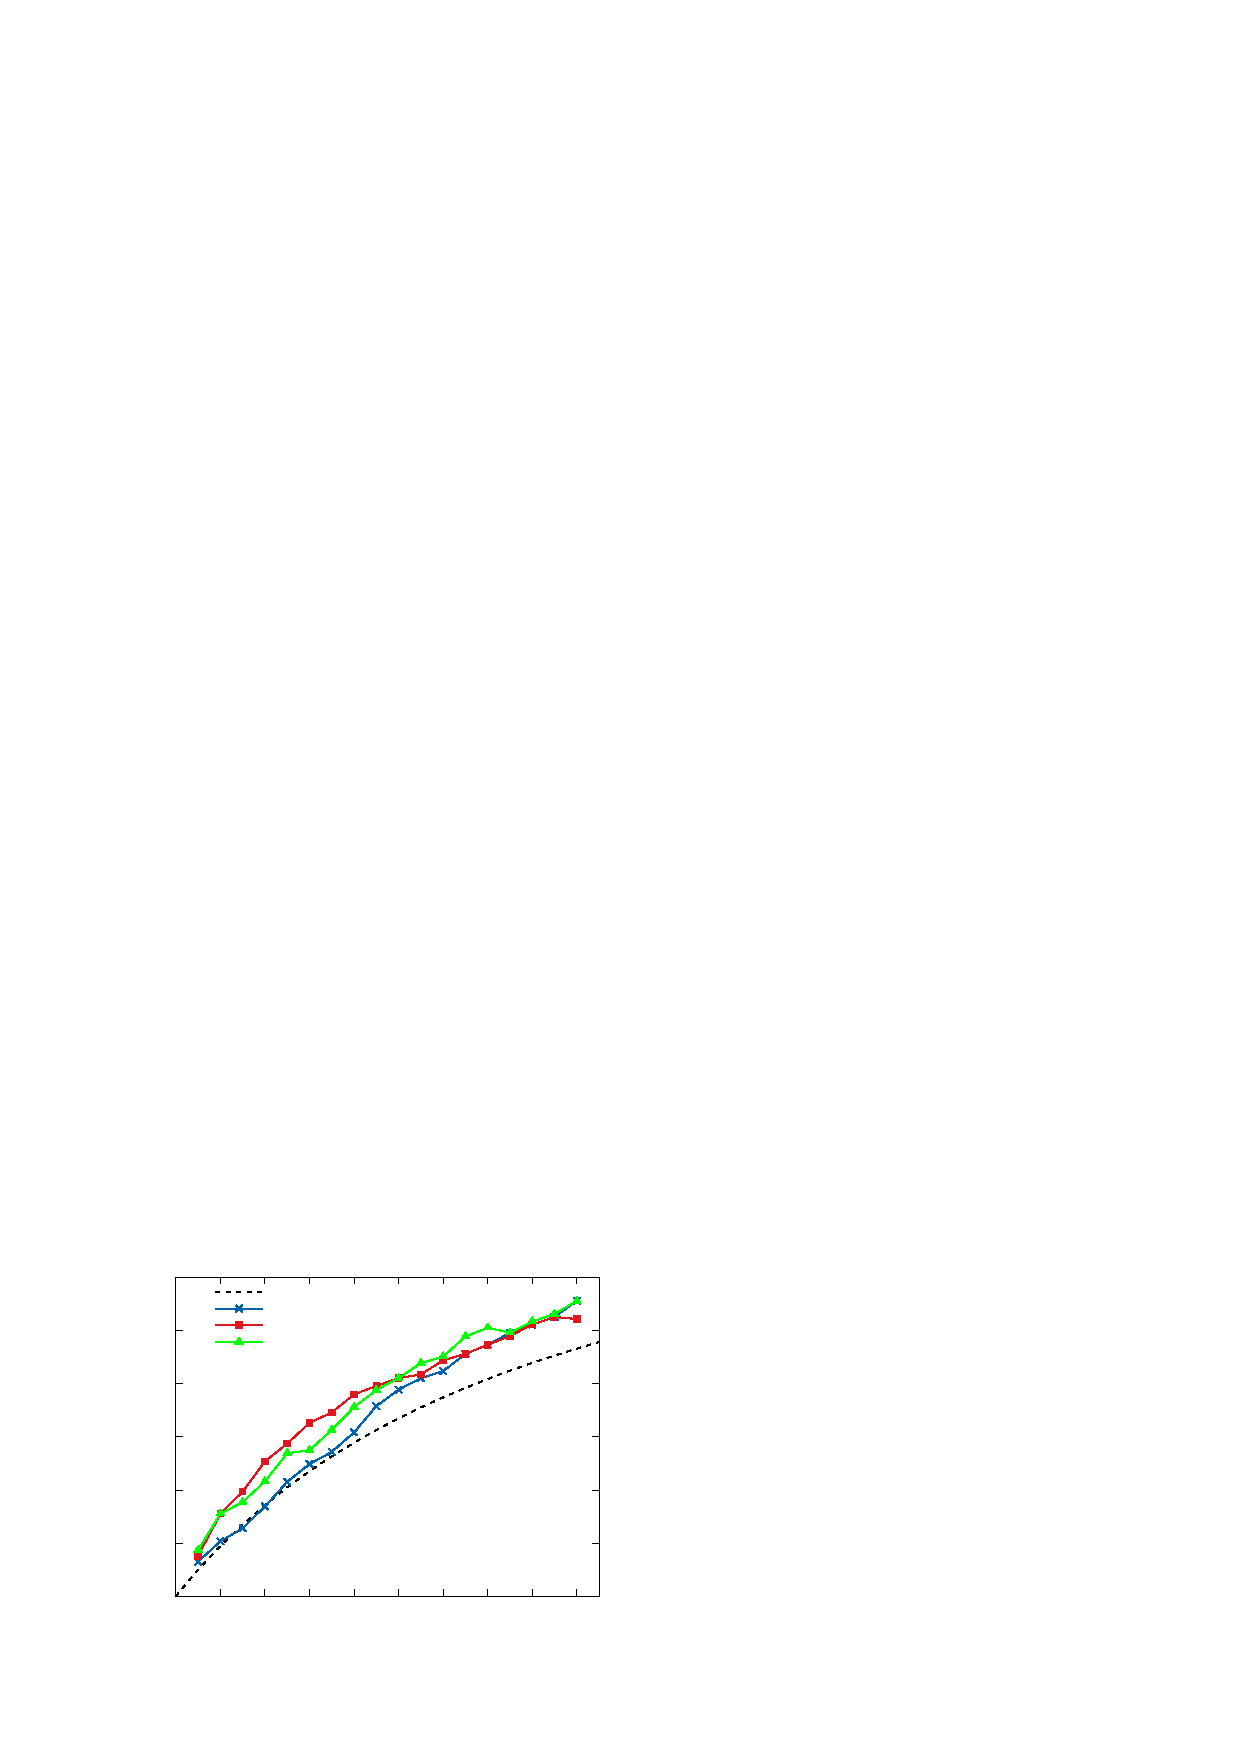
\includegraphics{f1atk}}%
    \gplfronttext
  \end{picture}%
\endgroup
}
		\caption{F1-score at top $k$}
		\label{fig:f1atk}
		
	\end{subfigure}
	\caption{The precision, recall and F1-score at top k of the 4 methods. (ER=Expected Random, PR=Popularity Ranking, LT=Linear Transform, TS=Translation Space)}
\end{figure*}
\subsection{Experimental Results}

%We introduce a baseline to compare with our three methods. In our baseline method, we sorted the named
%entity list by the total number of linking links to it in both English and Chinese corpus. It is based on
%the assumption that more frequent entities like public characters are usually more controversial.

\subsubsection{Entity Linking Accuracy}

In order to see the performance of our entity linking method, we randomly sampled 50 pieces of English news and Chinese news respectively.
On the whole, there are 1,530 links in English samples, 50 among which are incorrect. Chinese samples contain 436 links and there are
23 errors. We thus achieve accuracies of \textbf{96.7\%} and \textbf{94.7\%},
respectively.

\subsubsection{Word-embedding Results}

To evaluate the correctness of our word embedding results of entities, we
%randomly sampled \SH{number?} lots of entities and calculated
show qualitative results of high cosine similarity neighbors.
%We investigated top 20 terms for each of the sampled entities. The result is quite good.
To illustrate, Table~\ref{tbl:embd} shows the top similar entities of
``Adolf Hitler'' in the two cultures, including
similar semantic information with Benito Mussolini, Nazi Germany and the word ``dictator''.

\begin{table}[th]
\small
\centering
\caption{Top 7 most similar terms to the named entity ``Adolf Hitler'' by cosine similarity. (The Chinese terms in the table have already been translated into English. The words in italic are named entities in our vocabulary.) }
\label{tbl:embd}
\begin{tabular}{|c|c||c|c|}
\hline
\textbf{English Space} & \textbf{Sim.} & \textbf{Chinese Space} &
\textbf{Sim.}\\ \hline\hline
Hitler & 0.929 & \em{Nazi Germany}  & 0.869 \\ \hline
\em{Benito Mussolini} & 0.827 & Nazi  & 0.811 \\ \hline
Fuhrer & 0.817 & \em{Nazi Party}  & 0.769 \\ \hline

Stalin & 0.798 & Napoleon  & 0.753 \\ \hline
\em{Nazi Germany} & 0.790 & Stalin  & 0.729 \\ \hline
Nazi & 0.774 & \em{Benito Mussolini}  & 0.716 \\ \hline
\em{Heinrich Himmler} & 0.751 & dictator  & 0.704 \\ \hline
\end{tabular}
\end{table}

\subsubsection{Precision, Recall and F1-score at Top k}

%\BL{Figure 7 just need to tell the reader once that what colors means.}
We can regard our cross-cultural entity similarity mining experiment as a ranked retrieval problem.
Figure~\ref{fig:precisionatk} reports quantitative comparison of our two algorithms with the two baselines.
Note the accuracy of
 Expected Random Classifier baseline is fixed as  $173/379$ and its recall-at-k as $k/379$, shown as a dotted line.
%, though which we can also calculate the function of its F1-score.
In the figure, our two algorithms consistently outperform the two baselines, until $k$ reaches 150 where all algorithms converge.
Translational space performs comparably to Linear transform requiring seed annotation, and even outperforms when $k<20$ or $k>100$.
%\SH{Any good explanation why?}

%In Figure~\ref{fig:precisionatk}, we can conclude that our two algorithms outperform the two baselines significantly. Although our two algorithms and popularity ranking baseline all decrease at first and start to converge at $k=150$, there are still many differences among these three.
%Both the Translation Space and Popularity Ranking baseline decrease pretty much at first and then begin to rise up at $k=60$ thanks to the positive feedback of the delay reaction.
%However, the Linear Transformation converges more stably. Both of our algorithms are always higher than the two baselines.

Our algorithms, focusing on precision, are comparable in terms of recall with baselines as shown in
Figure~\ref{fig:recallatk},
such that in terms of F1-measure, we outperform the baselines in
%do not show much advantages than the two baseline.
%However, after observing
Figure~\ref{fig:f1atk}. %, we can say that our algorithms are better than baselines in all these three metrics.


Table~\ref{tbl:corr} reports the mean average precision (MAP)~\cite{schutze2008introduction}. Biased random as a baseline achieves 0.456, which is improved by our two proposed algorithms by 35.3\% and 34.2\% respectively.



\begin{table}[th]
\small
\centering
\caption{Performance comparison}
\label{tbl:corr}
\begin{tabular}{l|c}
       {\bf Method}   & {\bf MAP} \\ \hline
Biased Random & 0.456 \\ \hline
Popularity Ranking & 0.543 \\ \hline
Linear Transform&  0.612 \\ \hline
Translation Space& \textbf{0.617} \\
\end{tabular}
\end{table}


\begin{table}[h!]
	\small
	\centering
	\caption{Most culturally different named entities.}
	\label{tbl:list}
	\begin{tabular}{l|l}
		\textbf{Linear Transform} & \textbf{Translation Space} \\ \hline
		Bihar & Baltimore \\ \hline
		Sichuan & Human Rights Watch \\ \hline
		Gujarat & APEC \\ \hline
		China Central Television & Beijing\\ \hline
		West Bengal & Greenpeace \\ \hline
		Madhya Pradesh & China Central Television\\ \hline
		Korean Central News Agency & Korean Central News Agency\\ \hline
		Bharatiya Janata Party & African Union
		
		
	\end{tabular}
\end{table}

\subsubsection{The Most Culturally Different Entities}

Table~\ref{tbl:list} shows the most culturally different entities we mined from
%the large text through
our two algorithms. As discussed in Section 1, entities in the list include
entities located in China or neighboring countries (e.g., Bihar, Sichuan,
CCTV and Korean Central News Agency), for which the volume of interests is
significantly different in the two cultures. In the case of more common
entities such as Beijing, it carries more political connotations for
the westerners but is instead more of a cultural and geographic landmark
for the Chinese people, which shows different directions of interest.


%\BL{add the expected result in table 2}
%\KZ{Argue why we don't use MRR here. Because ultimately we are doing
%a classification/retrieval problem, not a ranking problem. We have
%large number of true positives, while MRR reward the true positives in
%the very top of the ranking much more than later in the rankings.}

